\chapter{Reconhecimento de Padrões e Aprendizado de Máquina}
\label{ch:ML}

Este capítulo é destinado à apresentação da fundamentação teórica dos conceitos gerais de reconhecimento de padrões e dos algoritmos de aprendizado de máquina utilizados neste projeto. Também são detalhados os processos utilizados no pré-processamento dos dados de treinamento (imagens) e na extração de atributos que estão relacionados ao desenvolvimento do sistema.

%na etapa de construção do banco de dados,

\section{Conceitos Gerais}

O príncipio sobre o qual o Aprendizado de Máquina opera é a indução, na qual, a partir de um conjunto de casos (exemplos) que tipificam o problema, são feitas generalizações e, então, decisões são tomadas baseadas nessa regra construída. Para tal, necessita-se de um conjunto de dados de treinamento, que desempenham o papel dos exemplos para indução e um modelo de Aprendizado de Máquina, que irá ser ajustado conforme padrões apresentados nos dados de treinamento.

Como já descrito brevemente no Capítulo \ref{ch:intro}, o aprendizado indutivo da máquina pode ocorrer como aprendizado supervisionado (\textit{supervised learning}) ou aprendizado não-supervisionado (\textit{unsupervised learning}). O último caracteriza-se por utilizar um conjunto de dados para os quais não existem classes pré-definidas, então, as classes são formadas durante o treinamento da máquina, sendo os domínios divididos naturalmente. Essa divisão é feita a partir da análise de padrões nos dados (imagens) como regiões com alta densidade relativa de pontos no espaço \citeC{perottoalvares2005}.

Já o aprendizado supervisionado, como no caso deste projeto, se dá com um conjunto de dados de treinamento que possuem classes já definidas e, portanto, tem-se uma estrutura na seguinte forma: entrada e saída desejada. As classes são apresentadas como rótulos de cada amostra do conjunto de dados e todo esse processo de aprendizado supervisionado é mostrado na Figura \ref{fig:supervised}, na qual o conjunto de exemplos rotulados apresentam a forma $(\boldsymbol{x_i}, y_i)$, em que $\boldsymbol{x_i}$ é o vetor de uma amostra e $y_i$ é seu rótulo. O classificador obtido por meio do algoritmo de aprendizado de máquina é denotado como $f$. Neste exemplo, tem-se um conjunto de $n$ dados, onde cada dado $\boldsymbol{x_i}$ possui $m$ atributos.

\begin{figure}[H]
 \centering
  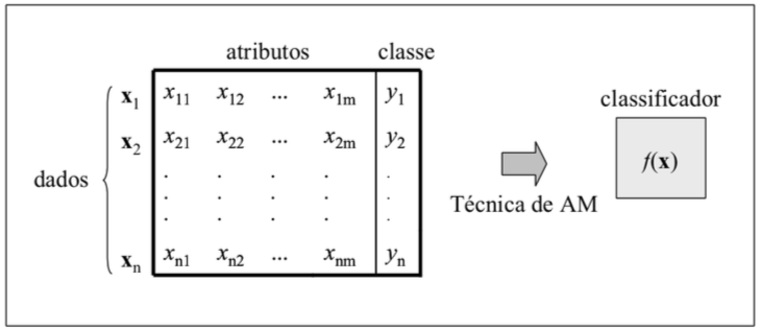
\includegraphics[width=0.8\linewidth]{figuras/supervisedLearning.pdf}
  \caption{Processo de treinamento de modelo classificador com aprendizado supervisionado \citeC{lorena2007}.}
  \label{fig:supervised}
\end{figure}

Os exemplos do conjunto de treinamento são representados como atributos em um vetor, sendo que cada atributo expressa uma característica do dado, a qual é utilizada no treinamento do modelo de aprendizado de máquina. Os tipos de atributos são o nominal e o contínuo. O primeiro tipo (nominal) gera um problema de classificação, no qual o objetivo é atribuir a cada vetor de entrada uma das categorias finitas (valores discretos). Este é o tipo de problema apresentado neste projeto. O tipo contínuo de atributo corresponde a um caso de regressão, em que à saída desejada é atribuída uma ou mais variáveis contínuas. Um exemplo é o problema de predição do preço de uma casa, que pode utilizar atributos como o tamanho e a localização da casa \citeC{Bishop2006}.

O classificador também utiliza uma função para descrever os dados. Sendo assim, é utilizada uma parte do conjunto de dados, denominada conjunto de teste, para mensurar o grau de desempenho do modelo de predição. Neste projeto, para avaliação do desempenho e da capacidade de generalização do modelo utiliza-se a técnica de Validação Cruzada (\textit{Cross Validation}). Nesta técnica, divide-se o conjunto total de dados em vários subconjuntos, sendo alguns utilizados para estimação dos parâmetros do modelo (etapa de treinamento) e outros, para a validação \citeC{kohavi1995}. Os três métodos mais populares de Validação Cruzada são: K-Pastas (\textit{K-Fold}), Substituição da Amostra (\textit{Holdout}) e Deixe-Um-De-Fora (\textit{Leave-One-Out}), sendo o primeiro escolhido para a implementação do sistema aqui apresentado \citeC{gonzalez2013}.

No método K-Pastas, o conjunto de dados é dividido aleatoriamente em $k$ subconjuntos, sendo um subconjunto destinado para teste e $k-1$ subconjuntos, para treinamento. O processo de treinamento do modelo classificador e de avaliação de seu desempenho é realizado $k$ vezes, sendo que, a cada vez que o processo é repetido, faz-se uma nova divisão do conjunto total em subconjuntos. Então, o desempenho final do classificador é obtido calculando-se a média de $k$ avaliações \citeC{schneider1997}.

%\section{Métodos Utilizados na Composição do Banco de Imagens e na Etapa de Pré-Processamento}

\section{Extração de Atributos}

Para o treinamento do algoritmo classificador são necessários atributos dos dados do conjunto de treinamento. A extração de atributos está relacionada com a redução da dimensionalidade de dados. Além de serem parâmetros descritivos do dado ao qual pertence, os atributos evitam que a quantidade de dados de entrada para o treinamento do modelo seja excessivamente grande, o que aumentaria o esforço computacional.

Desta forma, o problema de super-ajustamento (\textit{overfitting}) às amostras no treinamento pode ser evitado com a correta seleção de atributos.  O super-ajustamento pode ser causado por uma grande quantidade de variáveis no modelo, sendo definido como uma demasiada especialização nos dados de treinamento e, consequentemente, uma generalização ruim que gera uma baixa taxa de acerto para dados de entrada diferentes dos de treinamento \citeC{lorena2007}.

Também pode ocorrer um caso de sub-ajustamento (\textit{underfitting}), o que produz uma taxa de acerto que pode ser também considerada baixa para esta aplicação. O sub-ajustamento, por sua vez, é quando o modelo treinado não descreve bem o conjunto de dados de treinamento, apresentando baixa e insuficiente especialização em relação a esses dados. O sub-ajustamento em geral se deve à escolha de atributos pouco representativos para o tipo de análise pretendida.

Conclui-se, então, que a etapa de extração de atributos é importante para o bom desempenho do classificador. Neste projeto, a extração de atributos das imagens de entrada foi feita utilizando o operador Padrão Binário Local (LBP, \textit{Local Binary Pattern} em inglês). Os vetores de atributos são formados concatenando-se os histogramas das imagens resultados da aplicação do LBP, o qual é descrito a seguir.


\subsection{Padrão Binário Local (LBP)}

O operador LBP se popularizou devido à sua simplicidade computacional, que possui pouca sensibilidade à variação de iluminação e invariância à rotação. Esse operador, quando aplicado em uma imagem, substitui cada pixel (central) por um valor binário, que é obtido por meio da comparação desse pixel com seus vizinhos. Mais especificamente, forma-se uma matriz de nove pixels, no qual o pixel central é comparado com todos os oito pixels vizinhos ao pixel central. Para os pixels com valor maior do que o pixel central, atribui-se "1", caso contrário, atribui-se "0". Após esse processo, um número binário é gerado, considerando que a matriz foi avaliada em sentido horário, com o primeiro pixel sendo o bit menos significativo. Uma ilustração da aplicação do operador LBP em um pixel de uma imagem é apresentada na Figura \ref{fig:lbpTeoria}. Neste exemplo, qual o valor resultante gerado após a aplicação do LBP é 184 \citeC{do2012}. Em segundo momento na Figura \ref{fig:lbpTeoria}, mostra-se a imagem resultante após a aplicação do LBP.

\begin{figure}[H]
 \centering
  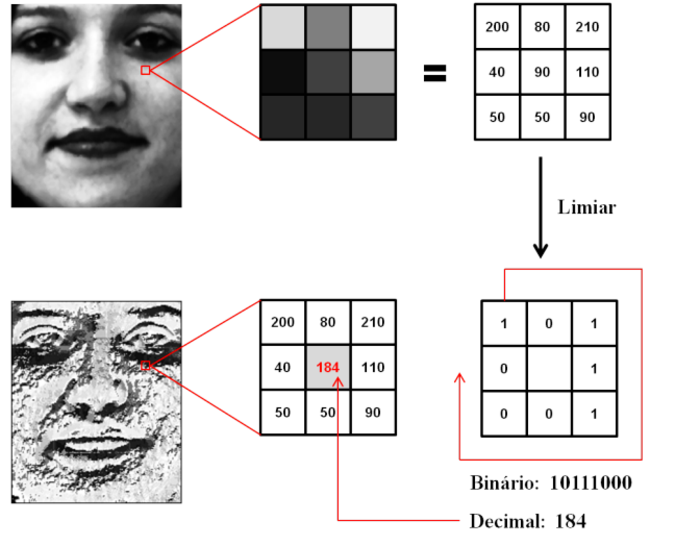
\includegraphics[width=0.65\linewidth]{figuras/lbpTeoria.pdf}
  \caption{Processo do operador LBP em um pixel \citeC{do2012}}
  \label{fig:lbpTeoria}
\end{figure}

Naturalmente, o LBP pode ser computado em áreas maiores do que 3x3 pixels. Neste caso, cria-se uma circunferência de raio $R$, que pode ser ajustado. Também se determina o número de pontos amostrais $P$ sobre a circunferência. A comparação se dá entre o pixel principal central e as posições amostradas no círculo com a imagem interpolada. Este procedimento é ilustrado ilustrado na Figura \ref{fig:lbpTeoria2} para alguns valores de P e R.


\begin{figure}[H]
 \centering
  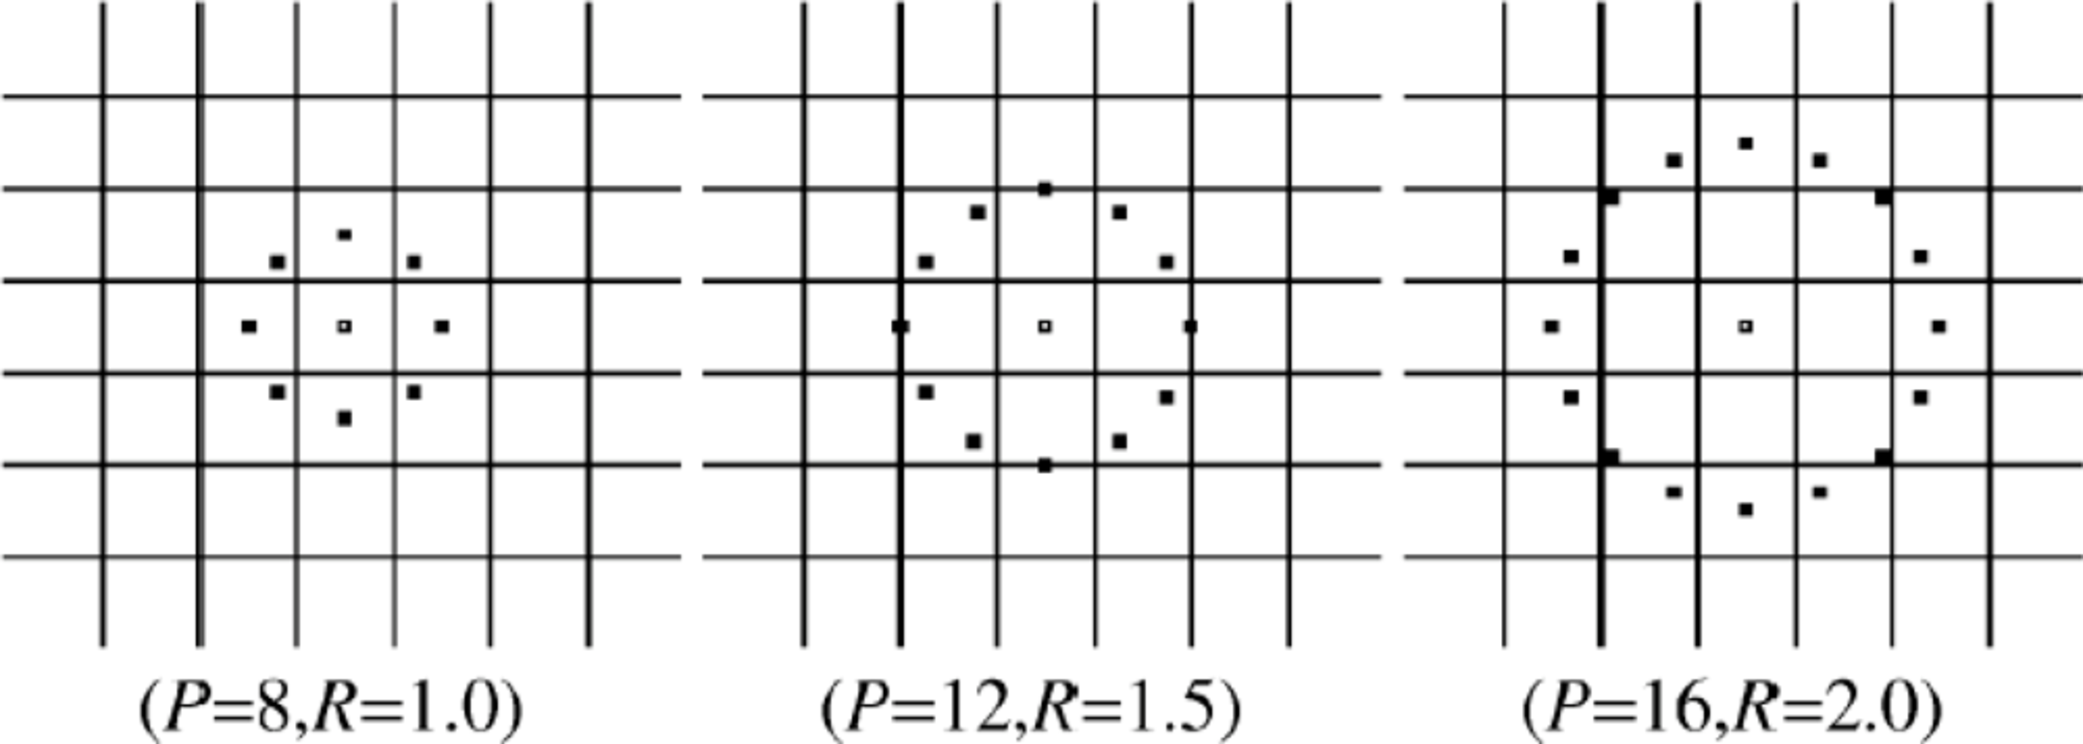
\includegraphics[width=0.65\linewidth]{figuras/lbpRP.pdf}
  \caption{Exemplo de operador LBP com diferentes valores de $P$ e $R$ \citeC{zhao2011}}
  \label{fig:lbpTeoria2}
\end{figure}

A seguinte equação define o operador LBP nos termos de $R$, $P$ e os valores em escala de cinza dos pixels da imagem:

\begin{equation}
\label{eq:eqLBP}
 LBP_{P,R}
   \begin{cases}
    \displaystyle\sum_{p=0}^{P-1}S(g_p - g_c)  & \quad \text{se número de transições} \leq 2 \\
    P+1  & \quad \text{caso contrário } \\
   \end{cases}
\end{equation}

 Sendo $g_c$ o valor do pixel central e $g_p$, o do pixel que está sendo comparado. Assim, obtém-se a sequência de valor binário $T_p={S(g_0 - g_c), ...,S(g_{P-1} - g_c)}$, em que $S(x) = 0$ se $x < 0$ e é igual a 1 caso contrário \citeC{muscipadroes}.

Para tornar o operador LBP invariante à rotação, pode-se modificar a ordem com que coleta-se os bits, de forma a alterar a sua representação binária. Mais especificamente, escolhemos como a primeira posição entre os pontos amostrais aquela que gera o menor valor final. Isso faz com que a possibilidade de valores para o LBP seja de 36 variações no total \citeC{prince2012}.

Pode também haver uma predominância da ocorrência de valores binários considerados uniformes, ou seja, aqueles em que são poucas, ou inexistentes, as transições de 0 para 1. Desta forma, a quantidade de classes de texturas pode ser reduzida quando agrupam-se todos os LBPs não-uniformes em uma única classe.

De forma geral, após o cálculo do LBP para todos os pixels da imagem, calcula-se o histograma desta nova imagem. O histograma é um descritor com a principal função de apresentar de forma compacta as características da imagem. O histograma usado para o LBP, enquanto uma função discreta, pode ser descrito pela seguinte equação:

\begin{equation}
\label{eq:eqHist}
  h(r_k)=n_k
\end{equation}

Onde $r_k$ é o valor de uma das classes do LBP e $n_k$ é a quantidade de pixels que apresentam o referido valor do LBP \citeC{gonzalezwoods2014}.

No entanto, é comum utilizar a versão normalizada do histograma que é descrita por:

\begin{equation}
\label{eq:eqHistNorm}
  p(r_k)=\frac{n_k}{MN}
\end{equation}

Em que M e N representam as dimensões da imagem.

Sendo assim, ao final do processo, todos os histogramas da imagem são concatenados ao final do processo, de forma a se tornarem um único vetor de atributos daquela imagem.

\section{Classificadores}

Os atributos extraídos das imagens do conjunto formam vetores, um para cada imagem, de forma a caracterizá-las. Esses são os dados de entrada para o modelo classificador. As características destes dados de entrada são analisados na fase de treinamento do modelo para ajustar o classificador, de forma que ele consiga realizar a classificação correta de novos dados de entrada.

Neste projeto, os modelos escolhidos para classificação no sistema foram: Máquina de Vetor de Suporte (SVM, em inglês \textit{Support Vector Machine}) em primeiro momento e, posteriormente, a Floresta Aleatória (\textit{Random Forest Classifier}). Ambos são apresentados mais detalhadamente nas seções seguintes.

\subsection{Máquina de Vetor de Suporte}

As Máquinas de Vetor de Suporte são um modelo de aprendizado com grande popularidade na comunidade de Aprendizado de Máquina. A SVM é utilizada em variadas aplicações, desde bioinformática ao reconhecimento de imagens, como é o caso desse projeto \citeC{mitchell1997} \citeC{noble2004} \citeC{kim2002}.

Intrinsicamente, a SVM é um modelo de classificação binária em problemas de aprendizado supervisionado (\textit{supervised learning}). Concedido um conjunto de dados para treinamento, todos especificados como pertencendo a uma das duas categorias, o treinamento do algoritmo SVM gera um modelo que irá classificar novos dados como sendo de uma categoria ou de outra.

A SVM baseia-se em um mapeamento de todos os dados de treinamento, representando-os como pontos em um espaço. Os exemplos para treinamento são divididos nesse espaço de acordo com sua categoria de tal forma que os dois conjuntos de pontos estejam distanciados pelo maior espaçamento possível (d), como ilustrado na Figura \ref{fig:svmDist}. Sendo assim, um novo dado, quando fornecido ao sistema, é mapeado nesse mesmo espaço e a predição de sua classe é feita de acordo com a sua localização no espaço, que foi gerado no treinamento do modelo.

\begin{figure}[H]
 \centering
  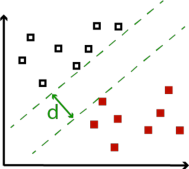
\includegraphics[width=0.4\linewidth]{figuras/svmDist.pdf}
  \caption{Ilustração da distância dos subconjuntos de dados de treinamento mapeados no espaço pelo modelo SVM.}
  \label{fig:svmDist}
\end{figure}

Em sua versão linear, a SVM pode ser classificada como "Margens Rígidas" ou "Margens Suaves". Em ambos casos, definem-se fronteiras lineares (para aplicação do limiar de decisão) no conjunto de dados que aprensentam perfil linearmente separável. As margens são utilizadas na SVM para encontrar a solução de classificação para os subconjuntos de forma que o erro de generalização seja o menor possível. Desta forma, as margens são definidas como a menor distância entre o hiperplano (fronteira) de decisão e qualquer uma das amostras de treinamento \citeC{Bishop2006}.

No entanto, apesar de não se aplicar a este projeto, a SVM também pode ser empregada em problemas em que os dados de treinamento não são rotulados, ou seja, em caso de aprendizado não-supervisionado (\textit{unsupervised learning}). Para tal, há uma versão distinta da SVM que funciona baseada no mapeamento dos dados em um espaço. No entanto, inicialmente realiza-se um processo para encontrar as conexões naturais entre os dados de entrada, formando grupos de acordo com o grau de similaridade apresentado entre eles, para então distribuí-los no espaço. Essa técnica é um algoritmo de aglomeração (\textit{clustering}) conhecido como \textit{Support Vector Clustering} \citeC{ben2001}.

\subsubsection{SVM com Margens Rígidas}

Pode-se definir um conjunto de dados de treinamento \textit{C}, composto de dados \textit{$x_i$} $\in$ X, no qual \textit{i $=$ 1, ..., n} e X é o espaço de dados, cujos rótulos de categoria são \textit{$y_i$} $\in$ Y, onde Y = \{$-$1,$+$1\}. Sendo assim, o conjunto \textit{C} é dito linearmente separável caso possa-se criar um hiperplano tal que os subconjuntos de dados com valor $-$1 seja separado do subconjunto de dados $+$1 \citeC{lorena2007}.

A seguinte equação, representa um hiperplano qualquer e divide o espaço dos dados de treinamento em duas regiões, uma para representar $-$1 e outra, $+$1,

\begin{equation}
\label{eq:eqHiper}
 f(x)= \boldsymbol{w}\cdot \boldsymbol{x} + b = 0
\end{equation}


Desta forma, define-se uma função \textit{$g(x)$} como a função sinal de \textit{$f(x)$} que irá ser o padrão para a classificação de novos dados de entrada, dada pela seguinte equação:


\begin{equation}
\label{eq:eqSgn}
 g(x) = sgn(f(x)) =
   \begin{cases}
    +1       & \quad \text{se } w\cdot x + b \text{ } $>$ \text{ } 0\\
    -1  & \quad \text{se } w\cdot x + b \text{ } $<$ \text{ } 0\\
   \end{cases}
\end{equation}

na qual $\boldsymbol{w}$ é o vetor normal ao hiperplano criado.

Para $f(x) = 0$, a distância entre um ponto no espaço (amostra) e o hiperplano definido é dada por $|f(x)| \mathbin{/} ||w||$. Além disso, deve existir pelo menos um conjunto de parâmetros $\boldsymbol{w}$ e \textit{b} que satisfaça \textit{g(x)}, ou seja, tal que \textit{$y_i$ $\cdot$ $f(x_i)$ $>$ 0}. Sendo assim, pode-se definir a distância entre uma amostra $x_i$ qualquer e o hiperplano escolhido como na seguinte equação:

 \begin{equation}
\label{eq:eqDist}
  \frac{y_i \cdot f(x_i)}{||\boldsymbol{w}||} = \frac{y_i(\boldsymbol{w} \cdot x_i + b)}{||\boldsymbol{w}||}.
\end{equation}

As margens ($H_1$ e $H_2$) são definidas, em primeiro momento, mediante a distância perpendicular entre a fronteira de decisão e aquele que é o ponto mais próximo de todas as amostras dos dados de treinamento, como mostra a parte \textit{a} da Figura \ref{fig:marginSVM}. Posteriormente, as margens são maximizadas escolhendo-se a sua localização, tomando como base as amostras que se encontram mais próximas do hiperplano separador, como destacado na parte \textit{b} da Figura \ref{fig:marginSVM}. Essas amostras são denominadas Vetores de Suporte (\textit{support vectors}), dando nome à técnica de aprendizado. Para maximizar a distância entre os vetores de suporte e o hiperplano separador ($f(x) = 0$), deve-se otimizar os parâmetros $\boldsymbol{w}$ e \textit{b}, que são ajustados durante o treinamento do modelo \citeC{rosebrock2017}.

\begin{figure}[H]
 \centering
  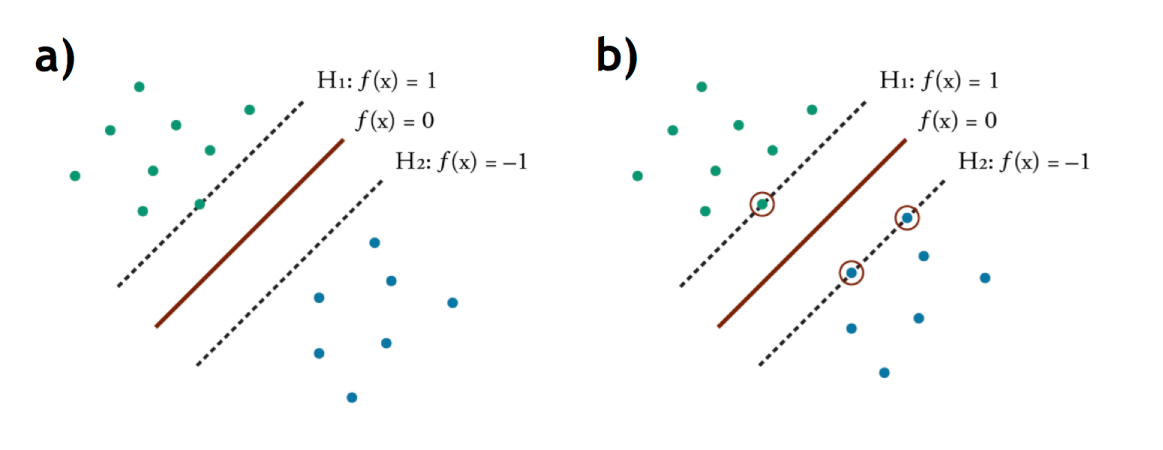
\includegraphics[width=0.9\linewidth]{figuras/marginSVM.pdf}
  \caption{Ilustração do hiperplano separador e do estabelecimento das margens ($H_1$ e $H_2$) no espaço em que os dados de treinamentos estão mapeados.}
  \label{fig:marginSVM}
\end{figure}

Realizando um escalonamento, a partir de uma mesma constante em termos de $\boldsymbol{w}$ e em \textit{b} não altera-se a distância dos pontos $x_i$ em relação ao hiperplano separador, a expressão $y_i(\boldsymbol{w} \cdot x_i + b)$ pode ser considerada unitária. Desta forma, a distância mínima entre o hiperplano e os dados de treinamento é de $1/||w||$. Busca-se, então, maximizar essa distância com a minimização de $||w||$, valendo-se do problema de otimização na expressão seguinte

\begin{equation}
\label{eq:eqMin}
  \text{min}\{\frac{1}{2}||\boldsymbol{w}||^2\},
\end{equation}

onde são consideradas as seguintes restrições

\begin{equation}
\label{eq:eqRestrição}
  \text{Restrições: } y_i(\boldsymbol{w} \cdot x_i + b) \geq 1, i \in (1,n)
\end{equation}

de forma a garantir que não haverão dados de treinamento entre as margens de separação de classes, daí então a nomenclatura "margens rígidas" \citeC{lorena2007}.

Esta é uma importante propriedade da SVM, tornando a determinação dos parâmetros do modelo uma otimização convexa, na qual a solução mínima é obrigatoriamente a solução global \citeC{Bishop2006}.

Para solucionar o problema de otimização da equação \ref{eq:eqMin}, pode ser utilizada uma função Lagrangiana, associando parâmetros $a_i$ (multiplicadores de Lagrange) e tornando suas derivadas parciais nulas. A resolução completa deste problema pode ser encontrada nas referências \citeC{Bishop2006} e \citeC{lorena2007}. Valendo-se do resultado dessa operação, tem-se a definição da função utilizada para a classificação dos dados que serão fornecidos ao sistema, dada pela seguinte equação

\begin{equation}
\label{eq:eqSVM}
  g(x) = sgn(f(x)) = sgn\left(\displaystyle\sum_{i=1}^{n}a_iy_ik(\boldsymbol{x},\boldsymbol{x_i})+b\right)
\end{equation}

sendo a função sinal do resultado da função de Lagrange aplicada nesse caso.

Pode-se perceber que na Equação \ref{eq:eqSVM} empregou-se o conceito de \textit{kernel} na resolução final do problema de otimização. Define-se a função \textit{kernel} como $k(x,x') = \phi(\boldsymbol{x})^T\phi(\boldsymbol{x'})$, na qual $\phi(\boldsymbol{x})$ indica um mapeamento, ou transformação, para um determinado espaço de características (\textit{feature space}), $\phi:X\mapsto\eth$. Apesar de, com o uso da função \textit{kernel} na formulação, o esforço computacional tornar-se mais elevado, dá-se flexibilidade ao modelo que pode ser reformulado usando diferentes tipos de \textit{kernel} e, então, pode ser aplicado em outros casos nos quais a dimensionalidade excede o número de amostras de treinamento \citeC{Bishop2006}.

\subsubsection{SVM com Margens Suaves}

A SVM com Margens Suaves é uma adaptação da versão do algoritmo com Margens Rígidas para que o aprendizado seja mais eficiente em casos de dados reais, os quais, comumente, não se apresentam conjuntos de dados estritamente bem comportados, ou seja, linearmente separáveis. Com essa versão da SVM, propõe-se lidar com conjuntos de treinamento mais gerais. Para isso, exceções às restrições apresentadas na expressão \ref{eq:eqRestrição}. Sendo assim, são estabelecidas variáveis de folga ($\xi_i$, $i \in (1,n)$) e são adicionadas ao problema e a equação \ref{eq:eqRestrição} é modificada para:

\begin{equation}
\label{eq:eqSuave}
 y_i(\boldsymbol{w} \cdot x_i + b) \geq 1 - \xi_i, \text{ } \xi_i > 0, \text{ } i \in (1,n).
\end{equation}

O efeito dessa modificação é que, devido a essa folga adicional, alguns pontos dos dados de treinamento podem permancer entre as margens $H_1$ e $H_2$. Por outro lado, isto pode gerar erros de classificação \citeC{lorena2007}.

A forma de desenvolvimento do modelo é similar à SVM com Margens Rígidas, ou seja, também emprega-se a função de Lagrange, anulando suas derivadas parciais. No entanto, os parâmetros multiplicadores de Lagrange $a_i$ sofrem modificações. A equação \ref{eq:eqMin} é, nesse caso, alterada:

\begin{equation}
\label{eq:eqMinErro}
  \text{min}\{\frac{1}{2}||\boldsymbol{w}||^2\ + K\displaystyle\sum_{i=1}^{n}\xi_i\}.
\end{equation}

Sabe-se que um erro no conjunto de treinamento é indicado por $\xi_i > 1$, portanto, para que o erro gerado por $\xi_i$ seja minimizado, no qual a constante \textit{K} é um termo de regularização à minimização dos erros no conjunto de treinamento.

Como no caso anterior, os pontos denominados Vetores de Suporte são aqueles em que a condição $a_i > 0$ é satisfeita. Porém, neste caso, há outros tipos de Vetores de Suporte, denominados livres e limitados, que atendem às equações a seguir

\begin{equation}
\label{eq:eqCondicaoMarg1}
 a_i(y_i(\boldsymbol{w} \cdot \boldsymbol{x_i} + b) - 1 + \xi_i) = 0,
\end{equation}

\begin{equation}
\label{eq:eqCondicaoMarg2}
 (K - a_i)\xi_i = 0.
\end{equation}



Os vetores de suporte chamados livres são aqueles que se encontram exatamente em cima da margem, obedecendo $a_i \leq K$ e $\xi_i = 0$. Já os vetores de suporte limitados possuem $a_i = K$ e podem ser erros ($\xi_i > 1$) ou pontos classificados corretamente ($0 <\xi_i \leq 1$), porém, se localizando entre as margens. Esses vetores são ilustrados na Figura \ref{fig:margemSuave}.


\begin{figure}[H]
 \centering
  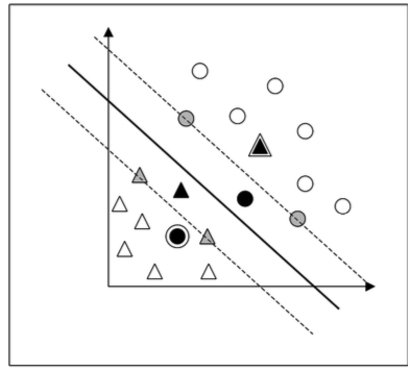
\includegraphics[width=0.4\linewidth]{figuras/margemSuave.pdf}
  \caption{Ilustração dos tipos de vetores de suporte: livres (cinza) e limitados (preto) \citeC{lorena2007}.}
  \label{fig:margemSuave}
\end{figure}

Em conclusão, obtém-se a mesma equação de classificação do modelo anterior (equação \ref{eq:eqSVM}), porém os parâmetros $a_i$ são calculados de forma distinta, com restrições que dependem da constante \textit{K}.

\subsubsection{SVM não-linear}

Apesar do modelo SVM com Margens Suaves ser mais abrangente do que aquele com Margens Rígidas, este modelo corresponde a um modelo de separação de categorias no qual um hiperplano é obtido, ou seja, é necessária uma característica linear na distribuição dos dados. No entanto, em aplicações reais, em alguns casos pode não ser possível seprar o subconjunto de dados por um hiperplano, como exemplificado na Figura \ref{fig:svmNL}.

\begin{figure}[H]
 \centering
  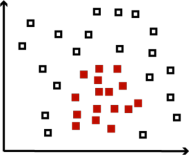
\includegraphics[width=0.35\linewidth]{figuras/svmNL.pdf}
  \caption{Ilustração de conjunto de dados de treinamento que não é linearmente separável}
  \label{fig:svmNL}
\end{figure}

Desta forma, atentando-se para a utilização da função \textit{kernel} (ver equação \ref{eq:eqSVM}), percebe-se que é possível empregar a SVM em uma classificação não linear, empregando um "truque de \textit{kernel}" { }(\textit{kernel trick}) que se resume em mapear os dados de entrada em um espaço com dimensão superior, denominado espaço de atributos (\textit{feature space}), como apresentado na Figura \ref{fig:svmKernel} \citeC{shawe2004} \citeC{boser1992}. Neste caso, observa-se $\phi:X\mapsto\eth$, no qual $\eth$ é o novo espaço de características. O bom desempenho do classificador depende de uma escolha apropriada de $\phi$, para que uma divisão linear nos dados de treinamento possa ser realizada.

\begin{figure}[H]
 \centering
  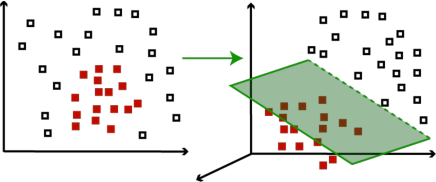
\includegraphics[width=0.75\linewidth]{figuras/svmKernel.pdf}
  \caption{Ilustração de mapeamento de conjunto de dados de treinamento em novo espaço de características a partir da utilização de função \textit{kernel}, possibilitando a divisão linear entre as categorias.}
  \label{fig:svmKernel}
\end{figure}

Segundo o teorema de Cover, para que os dados mapeados para o novo espaço de características tenham alta probabilidade de serem linearmente separáveis, duas condições devem ser satisfeitas \citeC{cover1965}. Primeiramente, a transformação ($\phi$) deve ser não-linear e, em segundo lugar, a dimensão do espaço de características deve ser suficientemente alta.

No processo de treinamento, ocorre o mapeamento dos dados de treinamento para o espaço de característicias aplicando-se $\phi$ no conjunto de dados. Com o objetivo de obter um nível relativamente baixo de ruídos, emprega-se a SVM com Margens Suaves. Após isso, as equações para otimização são calculadas, com a aplicação do operador $\phi$. Sendo assim, o classificador é o descrito na equação \ref{eq:eqSVM}.

Comumente, aplica-se o \textit{kernel} sem necessarimente a determinação prévia do operador $\phi$, deixando-o como uma operação implícita durante o treinamento. Esse é mais um motivo para usar a função \textit{kernel}, uma vez que se trata de um operador com cálculo simples (produto escalar) que representa bem os espaços. Para garantir que as condições expostas nesta seção sejam cumpridas, utilzam-se alguns tipos de \textit{kernel} que satisfazem as condições de Mercer \citeC{lorena2007}. As condições de Mercer são satisfeitas em um \textit{kernel} caso ele gere matrizes $\boldsymbol{K}$, em que cada elemento é definido por $K_{i,j}=K(\boldsymbol{x_i},\boldsymbol{y_j})$, para todo $i,j = 1,...,n$. Todos os \textit{kernels} que foram utilizados neste projeto são apresentados na Tabela \ref{tab:svmkernel}.

\begin{table}[h]
 \centering
 \begin{tabular}{l|c|c}
    Tipo & Função $k(x,x')$ & Parâmetros\\
  \hline
  Linear &  $(\delta(x \cdot x') + \kappa)$ & $\delta,\kappa$ \\
  Polinomial &  $(\delta(x \cdot x') + \kappa)^d$ & $\delta,\kappa, d$  \\
  RBF & $\exp(\frac{-||x - x'||^2}{2\sigma^2})$ & $\sigma$ \\
  Sigmoidal & $\tanh(\delta(x \cdot x') + \kappa)$ & $\delta,\kappa$ \\
 \end{tabular}
 \caption{Funções \textit{kernel} e seus parâmetros, utilizadas neste projeto \citeC{lorena2007} e \citeC{martin2012}}
 \label{tab:svmkernel}
\end{table}

\subsubsection{SVM Multiclasse}

Apesar de se tratar de um classficador que é intrinsicamente binário, a SVM pode também ser aplicada em problemas que apresentem várias categorias. Para tal, foram desenvolvidas ao longos dos anos novas soluções para a multiclassificação a partir de combinações múltiplas do classificador binário explicitado previamente nesta seção. Alguns modelos de adaptação do SVM para variadas classes são Um-contra-um (OvO, do inglês \textit{one vs. one}), Gráfico Acíclico Dirigido (DAG, do inglês \textit{Directed Acyclic Graph}), Código de Correção de Erro de Saída (ECOC, do inglês \textit{Error Corrected Output Coding}) e Um-contra-todos (OvA, do inglês \textit{One vs. All}), sendo este último utilizado neste projeto.


Supondo que um conjunto de dados possui $m$ classes, empregando a abordagem Um-contra-todos, um total de $m$ classificadores binários SVM devem ser criados para efetuar a classificação de uma determinada categoria em relação às $m-1$ demais classes. Então, no momento de testes ou de classificação de novos dados, esses dados são classificados criando-se uma margem (limiar de decisão) a partir do hiperplano separador e a classe desse dado será aquela que possuir uma função de decisão com maior valor, que corresponde à SVM que possui a maior margem dentre os demais \citeC{pal2008} \citeC{Bishop2006}.

Sendo assim, para um problema deste tipo, devem ser determinados $m$ hiperplanos. Consequentemente, é necessária a solução de $m$ problemas de otimização, sendo que, em cada um deles, uma classe é separada das demais. Desta forma, esta é uma desvantagem dessa abordagem, já que, durante a fase de treinamento, este processo é computacionalmente oneroso. Ademais, supondo que todas as classes possuam uma quantidade igual de amostras para treinamento, já que a SVM se comporta como um classificador binário, uma classe terá bem menos amostras para treino do que a outra classe, apresentando uma razão de $1:(m-1)$ \citeC{pal2008}.



\subsection{Floresta Aleatória}

O método Floresta Aleatória foi inicialmente proposto por Breiman \citeC{breiman2001} e pode ser aplicado tanto em problemas de classificação, quanto em problemas de regressão. O modelo classificador consiste em um conjunto de árvores aleatórias de decisão que são criadas durante o processo de treinamento do modelo, sendo escolhidos aleatoriamente os atributos dentro do vetor de entrada fornecido ao classificador \citeC{guedessistema}.

Passa-se, então, para o cálculo individual da entropia pertencente aos atributos. O atributo que apresenta a maior entropia é escolhido como sendo o nó que será utilizado na separação de classes nesta determinada posição na árvore. No caso deste modelo, o resultado final de classificação é obtido por meio da soma ponderada de predições sugeridas por diferentes conjuntos de parâmetros pertencentes às variadas árvores que compõem a floresta \citeC{prince2012}.

O método Floresta Aleatória possui várias vantagens, dentre elas \citeC{breiman2001}:

\begin{enumerate}
\item É um modelo relativamente robusto a ruídos;
\item É simples e é facilmente implementada de forma paralela;
\item Nas diversas aplicações na área, este método tem apresentado um melhor desempenho que outros em relação ao índice de acerto de classificação, métodos tais como a SVM e as Redes Neurais Artificias \citeC{caruana2008}.
\end{enumerate}

\subsubsection{Árvores de Decisão}

As árvores de decisão são uma técnica utilizada para a construção de modelos de classificação, que distribuiem os exemplos em um número finito de categorias. A técnica realiza a análise de um atributo, realizando a subdivisão dos dados do conjunto.

Sua estrutura se assemelha à uma árvore invertida, começando por um nó raiz e se subdividindo em ramos e em outros nós, até chegar em suas folhas, que são os pontos finais do sistema. Os nós internos são os nós de decisão e realizam o teste de atributos. Cada ramo está relacionado ao valor do atributo e, por último, cada folha representa uma classe \citeC{neto2014}.

Em geral, constroi-se uma árvore de decisão com um conjunto de dados de entrada, a partir do qual o nó raiz é criado e, após a realização de um teste, divide-se a árvore em ramos. Esse processo de avaliação do nó e da divisão em ramos é realizado nos nós subsequentes também, continuando a ramificação da árvore. Esse processo é realizado até que se atinja uma folha, não havendo mais ramificação. Todo esse procedimento é realizado recursivamente para conjunto de dados \citeC{bosch2007}.

\subsubsection{Procedimento da Floresta Aleatória}

A técnica de Floresta Aleatória é composta por um conjunto de árvores de decisão, no processo de crescimento de cada árvore é usado algum tipo de técnica aleatória. O conjunto de dados completo é dividido em subconjuntos, que serão os dados iniciais fornecidos à cada árvore. A aleatoriedade pode ser empregada durante o processo de divisão do conjunto de dados e na seleção do teste de cada nó.

No algoritmo de Floresta Aleatória, as árvores são binárias e os testes para decisão em cada nó podem ser escolhidos de forma aleatória, independentemente dos dados, ou por meio de um algoritmo que escolhe o teste que separa de melhor forma as amostras de treinamento. Neste caso, faz-se uma avaliação de acordo com a seguinte equação

\begin{equation}
\label{eq:randomF}
 \Delta E =
 - \displaystyle\sum_{i}\frac{|Q_i|}{|Q|}E(Q_i)
\end{equation}

na qual $\Delta E$ é o ganho de informação, que é gerado quando um conjunto de dados $Q$ é dividido em subconjuntos $Q_i$.

$E(q)$ é a entropia apresentada na seguinte expressão

\begin{equation}
\label{eq:entropy}
 E(q) = - \displaystyle\sum_{j=1}^{N}p_jlog_2(p_j)
\end{equation}

na qual $p_j$ é a proporção dos exemplos em $q$ que pertencem à classe $j$. Todo esse processo é recursivo e seu critério de parada pode ser pré-determinado escolhendo-se a quantidade de estimadores que serão utilizados na floresta, como no caso deste projeto. Outro critério de parada que pode ser utilizado é avaliar quando um nó não recebe exemplos suficientes.

Neste classificador, utiliza-se o conceito de probabilidade a posteriori, que se trata de probabilidade condicional de determinado evento aleatório. Durante o processo de treinamento do modelo, a probabilidade a posteriori é calculada para cada classe $c$ em cada folha $l$, que pertence à determinada árvore $a$. Essa probabilidade pode ser calculada como mostra a seguinte equação

\begin{equation}
\label{eq:probabilidade}
 P_{a,l}(Y(I)=c) = \frac{N_{c,l}}{N_l}
\end{equation}

 sendo que $Y(I)$ é a classe $c$ de determinanda imagem $I$, $N_{c,l}$ é o número de imagens da classe $c$ que chegaram à folha $l$ e, por último, $N_l$ é o número do total de imagens que alcançaram a folha $l$ \citeC{bosch2007}.

O processo de treinamento, avaliando as imagens do conjunto de treinamento, é inicializado no nó raiz e, então, passa pelas árvores de decisão até atingir alguma folha. Sendo assim, a classe daquela imagem é definida tomando-se o argumento máximo da média artimética de todas as probabilidades a posteriori.

No capítulo seguinte, retrata-se a metodologia utilizada no desenvolvimento deste projeto, relatando os processos de composição do banco de imagens, bem como os estágios de pré-processamento, extração de atributos e de treinamento utilizando-se os classificadores descritos no presente capítulo.
% breiman2001
%The common element in all of these procedures is that for the kth tree, a random vector  k is generated, independent of the past random vectors  1,..., k−1 but with the same distribution; and a tree is grown using the training set and  k, resulting in a classifier h(x, k) where x is an input vector.

%For instance, in bagging the random vector   is  generated as the counts in N boxes resulting from N darts thrown at random at the boxes, where N is number of examples in the training set. In random split selection   consists of a number of independent random integers between 1 and K . The nature and dimensionality of   depends on its use in tree construction.
%After a large number of trees is generated, they vote for the most popular class. We call these procedures random forests.

%Definition 1.1. A random forest is a classifier consisting of a collection of tree-structured classifiers {h(x,  k ), k = 1, . . .} where the { k } are independent identically distributed random vectors and each tree casts a unit vote for the most popular class at input x.

%To improve accuracy, the randomness injected has to minimize the correlation ρ ̄ while maintaining strength. The forests studied here consist of using randomly selected inputs or combinations of inputs at each node to grow each tree.

%Advantages

%ii It’s relatively robust to outliers and noise.
%iii It’s faster than bagging or boosting.
%iv It gives useful internal estimates of error, strength, correlation and variable importance.
%v It’s simple and easily parallelized.

%SEÇAO 10 = MECANISMO
%FALAR SOBRE CART TBM (livro)




